\chapter[The Generalized Lambda Distribution]{The Generalized Lambda Distribution}\label{cap:gld}

\begin{flushright}
	\textit{``There are good reasons for using the GLD distribution \\
	methods... GLD fits have been used successfully in many fields ...\\
	Try the GLD first and stop there if the results are acceptable.''\\
	(Karian and Dudewicz, 2011)}
\end{flushright}


Fitting statistical distribution to data (real or simulated), is an important task in uncertainty quantification forward problem. When fitting data, one typically first selects a general class, or family, of distributions and then finds values for the distributional parameters that best match the observed data \cite{Lakhany2000}. One of this families is the Generalized Lambda Distribution (\textit{GLD}), originally proposed by Ramberg and Schmeiser in 1974, as a generalization of the Tukey's distribution (1947). The \textit{GLD} has tested 

In this chapter a review of the principal characteristics of the \textit{GLD}

\section{The Generalized Lambda Distribution}

The generalized lambda distribution is a continuous distribution defined in terms of it quantile function. 

\subsection{The Ramberg and Schmeiser Parametrization}\label{sub:rs_gld}
The Generalized Lambda Distribution (\textit{GLD}) was proposed by Ramberg and Schmeiser in 1974 as an extention of the Tukey's distribution. It is represented by the quantil function:
\begin{equation}\label{eq:rs_param}
Q_{RS}(y|\lambda)=Q_{RS}(y|\lambda_{1}, \lambda_{2}, \lambda_{3}, \lambda_{4})=\lambda_{1}+\frac{y^{\lambda_{3}}-(1-y)^{\lambda_{4}}}{\lambda_{2}}
\end{equation}
where $Q_{RS}=F^{-1}$ is the quantile function for probabilities $y$, wiht $y\in[0,1]$; $\lambda_{1}$ and $\lambda_{2}$ are the location and scale parameteres, and $\lambda_{3}$ and $\lambda_{4}$ determine the skewness and kurtosis of the $GLD(\lambda_{1}, \lambda_{2}, \lambda_{3}, \lambda_{4})$.

The probability density function of the \textit{GLD} at the point $x=Q_{RS}(y)$ is given by:
\begin{equation}\label{eq:rs_pdf}
f(x)=f(Q_{RS}(y))=\frac{\lambda_{2}}{\lambda_{3}y^{\lambda_{3}-1}+\lambda_{4}(1-y)^{\lambda_{4}-1}}
\end{equation}

In order to have a valid distribution function, the probability density function $f(x)$ need to be positive for all $x$ and integrates to one over the allowed domain:
\begin{equation}
f(x) \geqslant 0
\end{equation}
\begin{equation}
\int f(x)dx=1
\end{equation}

This impose complex constraints on the parameters and support regions of the \textit{RS} parameterization, as summarized in table \ref{tab:rs_conts} and figure \ref{fig:rs_regions}.

% Please add the following required packages to your document preamble:
% \usepackage{multirow}
\begin{table}[]
\centering
\caption{Support regions of the GLD and conditions on the parameters given by the RS parameterization to define a valid distribution function \cite{Karian2011}. The support regions are displayed in Fig. \ref{fig:rs_regions}. Note that there are no conditions on $\lambda_{1}$ to obtain a valid distribution.}
\label{tab:rs_conts}
\begin{tabular}{c|c|c|c|c|c}
\hline
Region             & $\lambda_{2}$         & $\lambda_{3}$      & $\lambda_{4}$      & Q(0)                                                 & Q(1)                                                 \\ \hline
\multirow{3}{*}{1} & \multirow{3}{*}{$<0$} & $<=-1$             & $>=1$              & \multirow{3}{*}{$-\infty$}                           & \multirow{3}{*}{$\lambda_{1}+\frac{1}{\lambda_{2}}$} \\
                   &                       & $-1<\lambda_{3}<0$ & $>1$               &                                                      &                                                      \\
                   &                       & \multicolumn{2}{c|}{$\frac{(1-\lambda_{3})^{1-\lambda_{3}}(\lambda_{4}-1)^{\lambda_{4}-1}}{(\lambda_{4}-\lambda_{3})^{\lambda_{4}-\lambda_{3}}}=\frac{-\lambda_{3}}{\lambda_{3}}$}            &                                                      &                                                      \\ \hline
\multirow{3}{*}{2} & \multirow{3}{*}{$<0$} & $>=1$              & $<=-1$             & \multirow{3}{*}{$\lambda_{1}-\frac{1}{\lambda_{2}}$} &                                                      \\
                   &                       & $>1$               & $-1<\lambda_{4}<0$ &                                                      & $\infty$                                             \\
                   &                       & \multicolumn{2}{c|}{$\frac{(1-\lambda_{4})^{1-\lambda_{4}}(\lambda_{3}-1)^{\lambda_{3}-1}}{(\lambda_{3}-\lambda_{4})^{\lambda_{3}-\lambda_{4}}}=\frac{-\lambda_{4}}{\lambda_{3}}$}            &                                                      &                                                      \\ \hline
\multirow{3}{*}{3} & \multirow{3}{*}{$>0$} & $>0$               & $>0$               & $\lambda_{1}-\frac{1}{\lambda_{2}}$                  & $\lambda_{1}+\frac{1}{\lambda_{2}}$                  \\
                   &                       & $=0$               & $>0$               & $\lambda_{1}$                                        & $\lambda_{1}+\frac{1}{\lambda_{2}}$                  \\
                   &                       & $>0$               & $=0$               & $\lambda_{1}-\frac{1}{\lambda_{2}}$                  & $\lambda_{1}$                                        \\ \hline
\multirow{3}{*}{4} & \multirow{3}{*}{$<0$} & $<0$               & $<0$               & $-\infty$                                            & $\infty$                                             \\
                   &                       & $=0$               & $<0$               & $\lambda_{1}$                                        & $\infty$                                             \\
                   &                       & $<0$               & $=0$               & $-\infty$                                            & $\lambda_{1}$                                        \\ \hline
\end{tabular}
\end{table}

\begin{figure}[H]
    \centering
    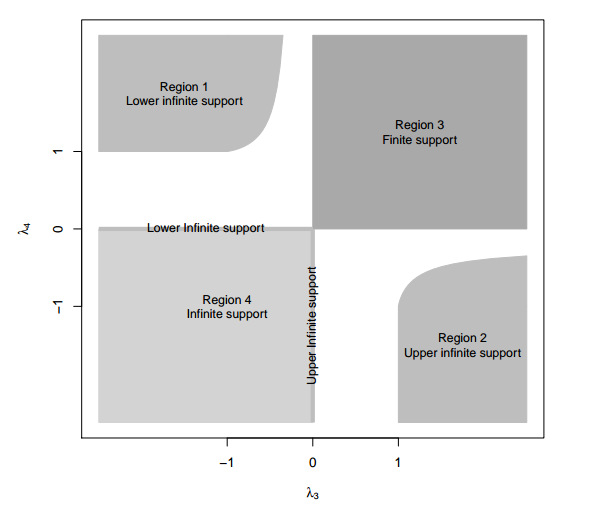
\includegraphics[width=0.8\textwidth]{img/gld/rs_regions.png}
    \caption{Support regions of the GLD in the RS parameterization that produce valid statistical
distributions.}
    \label{fig:rs_regions}
\end{figure}

\subsection{The FMKL Parameterization}\label{sub:fmkl_gld}
To circumvent the constraints on the \textit{RS} parameter values, Freimer, M., G. Mudholkar, G. Kollia and C. Lin (1988) introduced a new parameterization called \textit{FKML}, equation \ref{eq:fmkl_param}.

\begin{equation}\label{eq:fmkl_param}
Q_{FMKL}(y|\lambda_{1}, \lambda_{2}, \lambda_{3}, \lambda_{4})=\lambda_{1}+\frac{1}{\lambda_{2}}\left[\frac{y^{\lambda_{3}}-1}{\lambda_{3}} - \frac{(1-y)^{\lambda_{4}}-1}{\lambda_{4}} \right] 
\end{equation}

As in the previous parameterization, $\lambda_{1}$ and $\lambda_{2}$ are the location and scale parameters, but in this one $\lambda_{3}$ and $\lambda_{4}$ are the tail index parameters. The advantage over the previous parameterization is that the only constraint on the parameters is that $\lambda_{2}$ must be positive. Figure \ref{fig:fmkl_regions} displays the support regions of the \textit{GLD} in the \textit{FKML} parameterization, table \ref{tab:fmkl_conts}.

\begin{table}[]
\centering
\caption{Support regions of the \textit{GLD} given by the \textit{FMKL} parameterization \cite{Marcondes2018}.}
\label{tab:fmkl_conts}
\begin{tabular}{c|c|c|c}
\hline
$\lambda_{3}$ & $\lambda_{4}$ & Q(0)                                           & Q(1)                                           \\ \hline
$>0$          & $>0$          & $\lambda_{1}-\frac{1}{\lambda_{2}\lambda_{3}}$ & $\lambda_{1}+\frac{1}{\lambda_{2}\lambda_{4}}$ \\ \hline
$>0$          & $\leq0$         & $\lambda_{1}-\frac{1}{\lambda_{2}\lambda_{3}}$ & $\infty$                                       \\ \hline
$\leq0$         & $>0$          & $-\infty$                                      & $\lambda_{1}+\frac{1}{\lambda_{2}\lambda_{4}}$ \\ \hline
$\leq0$         & $\leq0$         & $-\infty$                                      & $\infty$                                       \\ \hline
\end{tabular}
\end{table}

\begin{figure}[H]
    \centering
    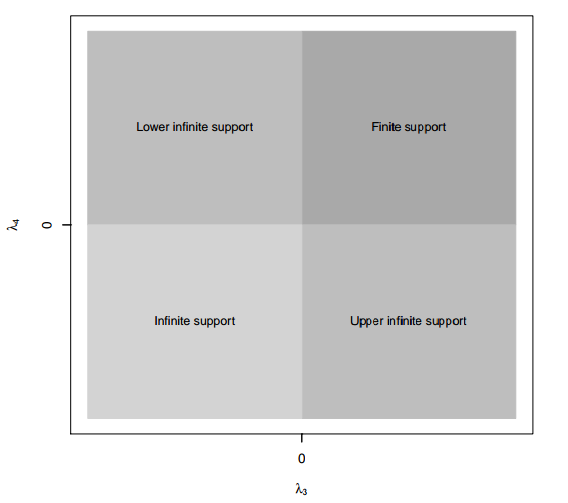
\includegraphics[width=0.8\textwidth]{img/gld/fmkl_regions.png}
    \caption{Support regions of the \textit{GLD} in the \textit{FMKL} parameterization that produce valid statistical
distributions.}
    \label{fig:fmkl_regions}
\end{figure}

The probability density function of the \textit{FMKL}-\textit{GLD} at the point $x=Q_{FMKL}(y)$ is given by \cite{Su2015}:
\begin{equation}\label{eq:fmkl_pdf}
f(x)=f(Q_{FMKL}(y))=\frac{\lambda_{2}}{y^{\lambda_{3}-1}+(1-y)^{\lambda_{4}-1}}
\end{equation}

Although both the \textit{RS} and \textit{FMKL} \textit{GLD} are generalizations of Tuckey's Lambda Distribution, they are not equivalent, so that the distribution fitted by one parametrization to a dataset differs in general from the one fitted by the other \cite{Marcondes2018}.

\subsection{Other Parameterizations}
One of the criticisms of the \textit{GLD} is that its skewness is expressed in terms of both tail indices $\lambda_{3}$ and $\lambda_{4}$. In one approach addressing this concern, a five-parameter \textit{GLD} was introduced by Joiner and Rosenblatt [1971], which, expressed in the \textit{FKML} parameterization, can be written as,
\begin{equation}\label{eq:jr_param}
Q_{JR}(y|\lambda_{1}, \lambda_{2}, \lambda_{3}, \lambda_{4})=\lambda_{1}+\frac{1}{2 \lambda_{2}}\left[(1-\lambda_{5})\frac{y^{\lambda_{3}}-1}{\lambda_{3}} - (1+\lambda_{5})\frac{(1-y)^{\lambda_{4}}-1}{\lambda_{4}} \right] 
\end{equation}

It has $\lambda_{1}$ and $\lambda_{2}$ as the location and scale parameters, and an asymmetry parameter, $\lambda_{5}$, which weights each side of the distribution and the two tail indices, $\lambda_{3}$ and $\lambda_{4}$. The conditions on the parameters are $\lambda_{2} > 0$ and $-1 < \lambda_{5} < 1$. The drawback of this parameterization is that the additional parameter can make the estimation of the parameter values even more difficult.

In \cite{Chalabi2012} the authors introduce a new parameterization of the \textit{GLD} that transform the \textit{FMKL} parameterization, equation \ref{eq:fmkl_param} in terms of an asymmetry and steepness parameter without adding a new variable. Its major advantage is that provides an intuitive interpretation of its parameters. A new \textbf{R} package called \textbf{gldist} was implemented with the new \textit{GLD} parameterization, along with the parameter estimation methods they present in his work. The problem with this parameterization is  that the \textbf{R} package was removed from the official repository because of the code is out of date.

\cite{Lodziensis2013}


\section{GLD Shapes}

\section{GLD fit common distributions}\label{sec:gld_fit_other}

\section{Numerical Methods to Fit the GLD to Data}
two different parameter estimation philosophies, 
\textbf{direct estimation methods}, such as least-squares estimation with order statistics [Ozturk and Dale, 1985] and with percentiles [Karian and Dudewicz, 1999, 2000; Fournier et al., 2007; King and MacGillivray, 2007; Karian and Dudewicz, 2003]; the methods of moments [Ozturk and Dale, 1982; Gilchrist, 2000], L-moments [Gilchrist, 2000; Karvanen and Nuutinen, 2008], and trimmed L-moments [Asquith, 2007]; and the goodness-of-fit method with histograms [Su, 2005] and with maximum likelihood estimation [Su, 2007]. On the other side, \textbf{stochastic methods} have been introduced with various estimators such as goodness-of-fit [Lakhany and Mausser, 2000] or the starship method [King and MacGillivray, 1999]. Moreover,
\cite{Lampasi2006}
Numerical maximum log likelihood estimation for generalized lambda distributions
\cite{Lakhany2000}
\cite{Fournier2007}
\cite{Marcondes2018}

\section{Fitting Mixture Distributions Using a Mixture of Generalized Lambda Distributions}
Esto esta en \cite{Tobergte2013}

Fitting the GLD and compare with the normal mixture \cite{Ning2008}

\section{GLD Random Variate Generation}
An important thing to take into account when we substitute the raw data produced as an output of a simulation process, by its \textit{PDF} is that those \textit{PDFs} need to allow us to reproduce the original data as close as possible. The outcome produced by a particular \textit{PDF} is known as random variate, its definition is:

\begin{defn} 
A \textbf{random variate} is a particular outcome of a random variable. The random variates which are other outcomes of the same random variable might have different values.
\end{defn}

Random variates are used when simulating processes driven by random influences. One of the important applications of the \textit{GLD} has been the generation of random variables for Monte Carlo studies \cite{Mustafa2016}.

This fact is justified by the following theorem, enunciated by Karian and Dudewicz (2010).

\begin{thm}
If $Q_{X}(y)$ is the percentile function of a random variable $X$, and $U$ is a uniform random variable
on $(0, 1)$ then $Q_{X}(U)$ has the same \textit{PDF} as does $X$.
\end{thm}

For a proof, also see p. 156 of Karian and Dudewicz (1999). The percentile function is not available in a closed (or easy-to-work-with) form for many of the most important distributions, such as the normal distribution. However, the GLD is (see sections \ref{sub:rs_gld} and \ref{sub:fmkl_gld}) defined by its p.f., which is a simple-to-calculate expression.

Thus, \textbf{r.v.s for a simulation study can easily be generated from any distribution that can be modeled by a GLD.}

\begin{exmp}
Suppose we have modeled an important \textbf{r.v.} by an approximate standard normal distribution $X$. We show in Section \ref{sec:gld_fit_other} that a close fit to the standard normal is available via the \textit{RS-GLD} with 
\begin{equation}
(\lambda_{1}, \lambda_{2}, \lambda_{3}, \lambda_{4}) = (0, 0.1975, 0.1349, 0.1349)
\end{equation}
and this \textit{GLD} has \textbf{p.f.} 
\begin{equation}
Q(y) = \frac{y^{0.1349}-(1-y)^{0.1349}}{0.1975}
\end{equation}
\end{exmp}

Thus, if $U_{1}, U_{2},...$ are independent uniform \textbf{r.v.s} on $(0, 1)$, then 
\begin{equation}\label{eq:random_variate}
Q(U_{1}), Q(U_{2}),...
\end{equation}
are independent and (approximately) $N(0, 1)$ \textbf{r.v.s} for the simulation study at hand.

This theorem means that, independently of the nature of the dataset (Normal, Exponential, etc.), when we fit a GLD to it, we can proceed similarly to the example above. That is, we just need to generate a stream of independent uniform \textbf{r.v.s} on $(0, 1)$, and then evaluate the equation \ref{eq:random_variate}. There are a number of good sources of independent uniform r.v.s on $(0, 1)$ \cite{Karian2011}. 

This is an important property of the \textit{GLD} that allow us to substitute the raw data by the four lambdas of the \textit{GLD} that best fit it (if the fit is a good one), with the warranty that if we need to go back, the \textit{GLD} could generate a good representation of the original data.


\section{GLD and Uncertainty Quantification}
\subsection{Related Works}
A solution to determining the reliability of products Using Generalized Lambda Distribution \cite{Movahedi2013}

Fundamental Reference \cite{Lampasi2006}

\subsection{Relevance of GLD in Uncertainty Quantification}
The use of the \textit{GLD} to quantify the uncertainty is justified because: 
\begin{itemize}
\item the \textit{GLD} fits the \textit{PDF} of a wide variety of datasets, including those that follow distributions such as normal, uniform, Student's t, U-shaped, exponential, etc;
\item no prior knowledge is needed to fit the \textit{GLD} to a dataset, which is practical and suitable for automatic and software procedures;
\item the \textit{PDF} is completely characterized by the four parameters of the \textit{GLD}, which represents a reduction in the amount of data that must be stored for post-processing;
\item the shape of the \textit{GLD} is governed by its parameters, so the \textit{GLDs} can be grouped  based on their shapes, which is especially useful for further queries; and
\item in cases where mixture of distributions are needed, \textit{GLD} mixtures could be a very good option.
\end{itemize}
\cite{Ning2008} 

\section{The GLDEX R package}\label{sec:gldex}
Last but not less important 

\section{Conclusions}

